% !TeX program = pdflatex
% Лабораторная работа №2. Разностные схемы для параболических уравнений.
\documentclass[12pt,a4paper]{article}

\usepackage[T2A]{fontenc}
\usepackage[utf8]{inputenc}
\usepackage[russian]{babel}

\usepackage{amsmath,amssymb}
\usepackage{graphicx}
\usepackage{booktabs}
\usepackage[left=2.5cm,right=2cm,top=2.5cm,bottom=2.5cm]{geometry}
\usepackage{caption}
\usepackage{xcolor}

% Таблицы: номер и заголовок сверху справа. Рисунки: подпись снизу по центру.
\captionsetup[table]{position=top,justification=raggedleft,
                     singlelinecheck=false,labelsep=period}
\captionsetup[figure]{position=bottom,justification=centering,
                      singlelinecheck=false,labelsep=period}

\definecolor{titlecol}{RGB}{130,22,22}

\newcommand{\norm}[1]{\left\|#1\right\|}
\renewcommand{\arraystretch}{1.15}

% Данные для титульного листа
\newcommand{\Discipline}{Численные методы}
\newcommand{\WorkKind}{ЛАБОРАТОРНАЯ РАБОТА №\,2}
\newcommand{\WorkTitleA}{Исследование разностных схем}
\newcommand{\WorkTitleB}{для параболических уравнений}
\newcommand{\StudentGroup}{5030102/30101}
\newcommand{\StudentName}{Андреев Даниил}
\newcommand{\TeacherLabel}{Проверил:}
\newcommand{\TeacherName}{}
\newcommand{\WorkYear}{2026}

\begin{document}

% Титульный лист
\begin{titlepage}
\color{titlecol}
\centering
\bfseries

\vspace*{18mm}

Министерство науки и высшего образования Российской Федерации\\[2mm]
{\large Санкт-Петербургский политехнический университет Петра Великого}\\[2mm]
Институт прикладной математики и механики\\[2mm]
Кафедра «Гидроаэромеханика и морская техника»

\vfill

{\Large \WorkKind}\\[3mm]
{\normalsize\mdseries по дисциплине «\Discipline»}\\[10mm]

{\large\mdseries \WorkTitleA\\[1.5mm] \WorkTitleB}

\vfill
\vfill

\hspace*{0.18\textwidth}%
\begin{minipage}{0.72\textwidth}
\mdseries
\begin{tabular}{@{}l@{\hspace{4mm}}l@{}}
Выполнил: & студент группы \StudentGroup\\
          & \StudentName\\[4mm]
\TeacherLabel & \TeacherName\\
\end{tabular}
\end{minipage}

\vfill

{\large Санкт-Петербург — \WorkYear}

\vspace*{10mm}
\end{titlepage}

\section{Постановка задачи}

Рассматривается краевая задача третьего рода для параболического
уравнения
\begin{equation}\label{eq:pde}
\frac{\partial u}{\partial t}-\rho(x)\,\frac{\partial^2u}{\partial x^2}
   = f(x,t),\qquad a\le x\le b,\quad 0\le t\le T,
\end{equation}
\begin{equation}\label{eq:rhocond}
0<\rho_{\min}\le\rho(x)\le\rho_{\max},\qquad \rho(x)\neq\mathrm{const},
\end{equation}
с начальным условием
\begin{equation}\label{eq:init}
u(x,0)=\varphi(x)
\end{equation}
и краевыми условиями третьего рода, которые ставятся так же, как в
работе~1:
\begin{equation}\label{eq:bc}
\begin{aligned}
-\alpha_a\,\frac{\partial u}{\partial x}(a,t)+\beta_a\,u(a,t)
  &=\gamma_a(t), && \beta_a\ge0,\\
 \alpha_b\,\frac{\partial u}{\partial x}(b,t)+\beta_b\,u(b,t)
  &=\gamma_b(t), && \beta_b\ge0,\qquad \alpha_a^2+\alpha_b^2\neq0 .
\end{aligned}
\end{equation}

\subsection{Тестовая задача с известным решением}

Чтобы можно было измерять погрешность, задача строится по известному
ответу. Решение берётся в виде
\begin{equation}\label{eq:ustar}
u^*(x,t)=v(x,t)\,w(x),\qquad
v(x,t)=p(x)\,e^{-kt}+1,\quad k>0,
\end{equation}
так что $v\to1$ и, значит, $u^*(x,t)\to w(x)$ при $t\to\infty$. Функция
$w$ --- установившееся состояние; оно удовлетворяет стационарной задаче,
которая получается из~\eqref{eq:pde} при $\partial u/\partial t=0$:
\begin{equation}\label{eq:stat}
\rho(x)\,\frac{d^2w}{dx^2}=g(x),\qquad g(x)=-\lim_{t\to\infty}f(x,t),
\end{equation}
с теми же краевыми условиями. В качестве $w$ взято решение из работы~1.

Такой вид решения показывает типичное поведение решений уравнений
параболического типа: убывание со временем и выход на установившийся
режим. Одновременно это иллюстрирует метод установления, когда
стационарная задача решается как нестационарная, доведённая до выхода на
установившееся состояние.

Подстановка $u^*$ в~\eqref{eq:pde}--\eqref{eq:bc} даёт согласованные
данные задачи:
\begin{equation}\label{eq:data_def}
f^*=\frac{\partial u^*}{\partial t}-\rho\,\frac{\partial^2u^*}{\partial x^2},
\qquad
\varphi^*(x)=u^*(x,0),
\end{equation}
\begin{equation}\label{eq:gamma_def}
\gamma_a^*(t)=-\alpha_a u^*_x(a,t)+\beta_a u^*(a,t),\qquad
\gamma_b^*(t)= \alpha_b u^*_x(b,t)+\beta_b u^*(b,t).
\end{equation}
Точное решение полученной задачи --- само $u^*$.

\subsection{Выбранные данные}

Принято
\begin{equation}\label{eq:data}
[a,b]=[0,2],\qquad
\rho(x)=1+\sin^2\frac{\pi x}{2},\qquad
p(x)=1+\frac{x}{2},\qquad k=3,
\end{equation}
\begin{equation}\label{eq:bcdata}
\alpha_a=1,\quad\beta_a=1,\qquad \alpha_b=1,\quad\beta_b=2,
\end{equation}
\begin{equation}\label{eq:w}
w(x)=x\sin2\pi x+e^{-x}\qquad\text{(решение из работы 1).}
\end{equation}

Условия задачи выполнены: $\rho_{\min}=1>0$, $\rho_{\max}=2$, функция
$\rho$ не постоянна; $\beta_a,\beta_b\ge0$ и
$\alpha_a^2+\alpha_b^2=2\neq0$.

Выбор $\rho$ не случаен. Максимум $\rho_{\max}=2$ достигается при $x=1$,
то есть во \emph{внутренней} точке отрезка. Граница устойчивости явной
схемы (п.~\ref{sec:stab}) определяется максимумом $\rho$ по тем узлам,
которые пересчитываются по явной формуле, а это внутренние узлы. Если бы
максимум достигался на краю, оценка $\tau\le h^2/(2\rho_{\max})$ была бы
завышенной и предсказанный порог не совпадал бы с наблюдаемым.

Так как $p'=1/2$ и $p''=0$, производные выписываются явно:
\begin{equation}\label{eq:pw}
(pw)'=\tfrac12 w+p\,w',\qquad (pw)''=w'+p\,w'' ,
\end{equation}
\begin{equation}\label{eq:derivs}
\begin{aligned}
u^*&=p\,w\,e^{-kt}+w, &\qquad
u^*_t&=-k\,p\,w\,e^{-kt},\\
u^*_x&=(pw)'e^{-kt}+w', &\qquad
u^*_{xx}&=(pw)''e^{-kt}+w'' ,
\end{aligned}
\end{equation}
откуда по~\eqref{eq:data_def}
\begin{equation}\label{eq:fstar}
f^*(x,t)=\bigl[-k\,pw-\rho\,(pw)''\bigr]e^{-kt}-\rho\,w'' ,
\qquad
\varphi^*(x)=\bigl(p(x)+1\bigr)w(x),
\end{equation}
а $\gamma^*_a,\gamma^*_b$ --- по~\eqref{eq:gamma_def}. Все данные задачи
зависят от времени только через множитель $e^{-kt}$; это используется в
программе, где функции от $x$ вычисляются один раз.

Предельный переход $t\to\infty$ в~\eqref{eq:fstar} даёт
$f^*\to-\rho w''$, то есть $g=\rho w''$ в~\eqref{eq:stat}, как и должно
быть.

\subsection{Момент установления}

Счёт по времени ведётся до момента установления $ust$, определяемого из
неравенства
\begin{equation}\label{eq:settle_def}
\frac{\norm{u(x,t)-u_{st}(x)}}{\norm{u_{st}(x)}}\le\delta,
\end{equation}
где $\delta$ --- малое число, а норма несеточная и подсчитывается при
фиксированном $t$. Здесь неравенство решается точно. Из~\eqref{eq:ustar}
\[
u^*(x,t)-w(x)=p(x)w(x)\,e^{-kt},
\]
множитель $e^{-kt}$ от $x$ не зависит и выносится из нормы, поэтому
\[
\frac{\norm{u^*(\cdot,t)-w}}{\norm{w}}
=e^{-kt}\,\frac{\norm{pw}}{\norm{w}}\le\delta
\quad\Longleftrightarrow\quad
t\ge\frac1k\ln\frac{\norm{pw}}{\delta\,\norm{w}} .
\]
Отсюда
\begin{equation}\label{eq:settle}
ust=\frac1k\,\ln\frac{\norm{pw}}{\delta\,\norm{w}} .
\end{equation}
Нормы берутся в $C[a,b]$ и считаются по мелкой сетке. При $\delta=10^{-3}$
получается $ust=2{,}5139$; это значение и принято за $T$.

\section{Разностные схемы}

\subsection{Сетка и обозначения}

Вводится прямоугольная равномерная по $x$ и по $t$ сетка
$\Omega_{h\tau}=\Omega_h\times\Omega_\tau$:
\[
\Omega_h=\{x_i=a+ih,\ i=0,\dots,M\},\quad h=\frac{b-a}{M};\qquad
\Omega_\tau=\{t_n=n\tau,\ n=0,\dots,N\},\quad N=\Bigl\lceil\frac T\tau\Bigr\rceil .
\]
Обозначения: $\rho_i=\rho(x_i)$, $f_i^n=f^*(x_i,t_n)$,
$v_i^n\approx u(x_i,t_n)$.

\subsection{Аппроксимация по пространству}

Во внутренних узлах вводится разностный оператор
\begin{equation}\label{eq:Lambda}
\Lambda v_i=\rho_i\,\frac{v_{i-1}-2v_i+v_{i+1}}{h^2},\qquad i=1,\dots,M-1 .
\end{equation}
Его погрешность получается из разложения Тейлора в точке $x_i$:
\[
u_{i\pm1}=u_i\pm h\,u_x+\frac{h^2}{2}u_{xx}\pm\frac{h^3}{6}u_{xxx}
          +\frac{h^4}{24}u_{xxxx}+O(h^5),
\]
при сложении члены с нечётными производными сокращаются, и
\begin{equation}\label{eq:d2}
\frac{u_{i-1}-2u_i+u_{i+1}}{h^2}=u_{xx}(x_i)+\frac{h^2}{12}u_{xxxx}(x_i)
   +O(h^4).
\end{equation}
Следовательно,
\begin{equation}\label{eq:Lambda_err}
\Lambda u_i=\rho(x_i)\,u_{xx}(x_i)
   +\rho(x_i)\frac{h^2}{12}u_{xxxx}(x_i)+O(h^4)
 =\rho\,u_{xx}+O(h^2),
\end{equation}
причём в остатке стоят только чётные степени $h$.

\subsection{Схема с весом}

Все три схемы задания записываются одной формулой --- схемой с весом
$\theta$:
\begin{equation}\label{eq:theta}
\frac{v_i^{n+1}-v_i^n}{\tau}
=\theta\bigl(\Lambda v^{n+1}+f^{n+1}\bigr)_i
+(1-\theta)\bigl(\Lambda v^{n}+f^{n}\bigr)_i,
\qquad i=1,\dots,M-1,
\end{equation}
\[
\theta=0 \;\text{--- явная},\qquad
\theta=1 \;\text{--- неявная},\qquad
\theta=\tfrac12 \;\text{--- симметричная}.
\]

Найдём порядок аппроксимации по времени. Обозначим $g=\rho u_{xx}+f$,
так что точное решение удовлетворяет $u_t=g$. Разложим обе части
в точке $t_{n+1/2}=t_n+\tau/2$:
\[
\frac{u^{n+1}-u^{n}}{\tau}=u_t(t_{n+1/2})+\frac{\tau^2}{24}u_{ttt}+O(\tau^4),
\]
\[
g^{n+1}=g(t_{n+1/2})+\frac{\tau}{2}g_t+\frac{\tau^2}{8}g_{tt}+O(\tau^3),
\qquad
g^{n}=g(t_{n+1/2})-\frac{\tau}{2}g_t+\frac{\tau^2}{8}g_{tt}+O(\tau^3),
\]
откуда
\[
\theta g^{n+1}+(1-\theta)g^{n}
=g(t_{n+1/2})+\Bigl(\theta-\frac12\Bigr)\tau\,g_t
 +\frac{\tau^2}{8}g_{tt}+O(\tau^3).
\]
Вычитая и пользуясь тем, что $u_t(t_{n+1/2})-g(t_{n+1/2})=0$, получаем
невязку
\begin{equation}\label{eq:theta_err}
\psi^{n+1/2}=\Bigl(\frac12-\theta\Bigr)\tau\,g_t+O(\tau^2).
\end{equation}
Член порядка $\tau$ обращается в нуль только при $\theta=1/2$: симметрия
весов относительно $t_{n+1/2}$ убирает первую поправку, как симметрия
центральных разностей убирала её в~\eqref{eq:d2}. Вместе
с~\eqref{eq:Lambda_err} это даёт порядок аппроксимации
\begin{equation}\label{eq:orders}
O(\tau+h^2)\ \text{для } \theta=0,1,
\qquad
O(\tau^2+h^2)\ \text{для } \theta=\tfrac12 .
\end{equation}

\subsection{Аппроксимация краевых условий со вторым порядком}
\label{sec:bc}

Производные в краевых условиях аппроксимируются трёхточечными
односторонними разностями. Разложения
\[
u_1=u_0+h\,u_x+\frac{h^2}{2}u_{xx}+\frac{h^3}{6}u_{xxx}+O(h^4),
\qquad
u_2=u_0+2h\,u_x+2h^2u_{xx}+\frac{4h^3}{3}u_{xxx}+O(h^4)
\]
комбинируются так, чтобы уничтожить $u_{xx}$:
\[
4u_1-u_2=3u_0+2h\,u_x-\frac{2}{3}h^3u_{xxx}+O(h^4),
\]
откуда
\begin{equation}\label{eq:onesided}
u_x(a)=\frac{-3u_0+4u_1-u_2}{2h}+\frac{h^2}{3}u_{xxx}(a)+O(h^3)
     =\frac{-3u_0+4u_1-u_2}{2h}+O(h^2),
\end{equation}
и симметрично на правом конце
\begin{equation}\label{eq:onesided_b}
u_x(b)=\frac{3u_M-4u_{M-1}+u_{M-2}}{2h}-\frac{h^2}{3}u_{xxx}(b)+O(h^3).
\end{equation}
Это и есть требуемая аппроксимация второго порядка. Подстановка
в~\eqref{eq:bc} даёт краевые уравнения
\begin{equation}\label{eq:bc_h}
\begin{aligned}
\Bigl(\frac{3\alpha_a}{2h}+\beta_a\Bigr)v_0^{n+1}
 -\frac{2\alpha_a}{h}v_1^{n+1}+\frac{\alpha_a}{2h}v_2^{n+1}
 &=\gamma_a(t_{n+1}),\\
\Bigl(\frac{3\alpha_b}{2h}+\beta_b\Bigr)v_M^{n+1}
 -\frac{2\alpha_b}{h}v_{M-1}^{n+1}+\frac{\alpha_b}{2h}v_{M-2}^{n+1}
 &=\gamma_b(t_{n+1}).
\end{aligned}
\end{equation}
Краевое условие --- алгебраическая связь, выполняющаяся в каждый момент
времени, поэтому оно ставится точно на слое $t_{n+1}$ и никакой
погрешности по $\tau$ не вносит: аппроксимация здесь только по $x$.
Благодаря этому все три схемы отличаются ровно весом $\theta$, и
сравнение между ними не искажается разной обработкой границы.

\subsection{Решение системы}

При $\theta=0$ схема~\eqref{eq:theta} явная:
\begin{equation}\label{eq:explicit}
v_i^{n+1}=(1-2r_i)v_i^n+r_i\bigl(v_{i-1}^n+v_{i+1}^n\bigr)+\tau f_i^n,
\qquad r_i=\frac{\tau\rho_i}{h^2},
\end{equation}
после чего $v_0^{n+1}$ и $v_M^{n+1}$ находятся из~\eqref{eq:bc_h}, где
все остальные значения уже вычислены.

При $\theta>0$ получается система линейных алгебраических уравнений
(СЛАУ) относительно $v^{n+1}$:
\begin{equation}\label{eq:slau}
-\theta r_i\,v_{i-1}^{n+1}+(1+2\theta r_i)\,v_i^{n+1}
-\theta r_i\,v_{i+1}^{n+1}
=v_i^n+\tau\bigl[(1-\theta)(\Lambda v^n+f^n)_i+\theta f_i^{n+1}\bigr]
\end{equation}
для $i=1,\dots,M-1$ вместе с~\eqref{eq:bc_h}. Матрица была бы
трёхдиагональной, если бы не элементы при $v_2$ и $v_{M-2}$ в краевых
строках. Они исключаются: из строки $0$ вычитается строка $1$,
умноженная на $k_0=c_{02}/B_1$, где $c_{02}=\alpha_a/(2h)$ ---
коэффициент при $v_2$ в строке~0, а $B_1=-\theta r_1$ --- коэффициент
при $v_2$ в строке~1; то же самое делается со строкой $M$ и строкой
$M-1$. Та же комбинация применяется к правым частям. Полученная
трёхдиагональная система решается методом прогонки.

Коэффициенты матрицы от номера слоя не зависят, поэтому прямой ход
прогонки (вычисление прогоночных коэффициентов) выполняется один раз
перед циклом по времени, а на каждом шаге остаются только пересчёт
правой части и обратный ход.

\subsection{Устойчивость}
\label{sec:stab}

\paragraph{Явная схема: принцип максимума.}
В~\eqref{eq:explicit} значение на новом слое --- линейная комбинация
значений на старом с коэффициентами $1-2r_i$, $r_i$, $r_i$, сумма
которых равна единице. Если все они неотрицательны, то
\[
\max_i|v_i^{n+1}|\le\max_i|v_i^n|+\tau\max_i|f_i^n|,
\]
то есть схема устойчива. Неотрицательность требует $1-2r_i\ge0$, то есть
$\tau\le h^2/(2\rho_i)$ для каждого пересчитываемого узла, а значит
\begin{equation}\label{eq:stabcond}
\tau\le\frac{h^2}{2\rho_{\max}} .
\end{equation}

\paragraph{Схема с весом: спектральный признак.}
Заморозим коэффициент ($\rho=\mathrm{const}$), положим $f=0$ и подставим
в~\eqref{eq:theta} гармонику $v_j^n=\lambda^n e^{\mathrm{i}\varphi j}$.
Так как
$\Lambda e^{\mathrm{i}\varphi j}
=-\frac{4\rho}{h^2}\sin^2\frac\varphi2\,e^{\mathrm{i}\varphi j}$,
то, обозначив $r=\tau\rho/h^2$ и $s=4r\sin^2(\varphi/2)\in[0,4r]$,
получаем
\[
\lambda-1=-s\bigl[\theta\lambda+(1-\theta)\bigr]
\quad\Longrightarrow\quad
\lambda=\frac{1-(1-\theta)s}{1+\theta s}.
\]
Неравенство $\lambda\le1$ выполнено всегда, так как $s\ge0$. Условие
$\lambda\ge-1$ равносильно
\[
1-(1-\theta)s\ge-1-\theta s
\quad\Longleftrightarrow\quad
(1-2\theta)\,s\le2 .
\]
При $\theta\ge1/2$ левая часть неположительна, и неравенство выполняется
при любом $s$: \emph{неявная и симметричная схемы безусловно устойчивы}.
При $\theta<1/2$ нужно $s\le2/(1-2\theta)$; так как $s\le4r$, достаточно
\[
r\le\frac{1}{2(1-2\theta)} .
\]
При $\theta=0$ это даёт $r\le1/2$, то есть $\tau\le h^2/(2\rho)$ ---
тот же результат~\eqref{eq:stabcond}, что и принцип максимума.

Максимально возможный шаг по времени для явной схемы обозначим
\begin{equation}\label{eq:tau0}
\tau_0=\frac{h_0^2}{2\rho_{\max}} .
\end{equation}

\section{Измерение погрешности}

Погрешность приближённого решения $v$ вычисляется по формуле
\begin{equation}\label{eq:eps}
\varepsilon=\frac{\norm{u-v}_{h\tau}}{\norm{u}_{h\tau}},
\qquad
\norm{u}_{h\tau}=\max_{t\in\Omega_\tau}\norm{u(t)}_h ,
\end{equation}
где $\norm{\cdot}_h$ --- норма на сетке $\Omega_h$. В работе взята
равномерная норма $\norm{y}_h=\max_i|y_i|$, так что
\begin{equation}\label{eq:eps_max}
\varepsilon=\frac{\max_{n,i}\bigl|u(x_i,t_n)-v_i^n\bigr|}
                 {\max_{n,i}\bigl|u(x_i,t_n)\bigr|} .
\end{equation}

Наряду с~\eqref{eq:eps_max} в работе используется \emph{контрольная}
оценка $\varepsilon_{\text{к}}$: то же отношение, но максимум берётся не
по $\Omega_\tau$, а по фиксированному набору из 101 равноотстоящего
момента на $[0,T]$, не зависящему от $\tau$; между слоями численное
решение восстанавливается линейной интерполяцией по $t$.

Необходимость второй оценки видна из определения. Сеточная область
$\Omega_\tau$ сама зависит от $\tau$: чем крупнее шаг, тем меньше в ней
слоёв. Погрешность $\norm{u(t)-v(t)}_h$ меняется со временем и имеет
максимум на переходном участке; при больших $\tau$ этот максимум может
просто не попасть ни в один слой, и формальная величина~\eqref{eq:eps_max}
окажется заниженной. Контрольная оценка от выбора $\tau$ в этом смысле
не зависит. Ниже, в п.~\ref{sec:taustar}, видно, что для симметричной
схемы расхождение между двумя оценками становится определяющим.

\section{Результаты}

Все расчёты проведены с данными~\eqref{eq:data}--\eqref{eq:w} до момента
установления $T=ust=2{,}5139$. Заданная точность
\begin{equation}\label{eq:eps0}
\varepsilon_0=5\cdot10^{-3} .
\end{equation}
Коэффициент $\rho(x)$ и точное решение $u^*(x,t)$ показаны на
рис.~\ref{fig:rho} и~\ref{fig:exact}; видно убывание со временем и выход
на установившийся режим $w(x)$.

\begin{figure}[htbp]
\centering
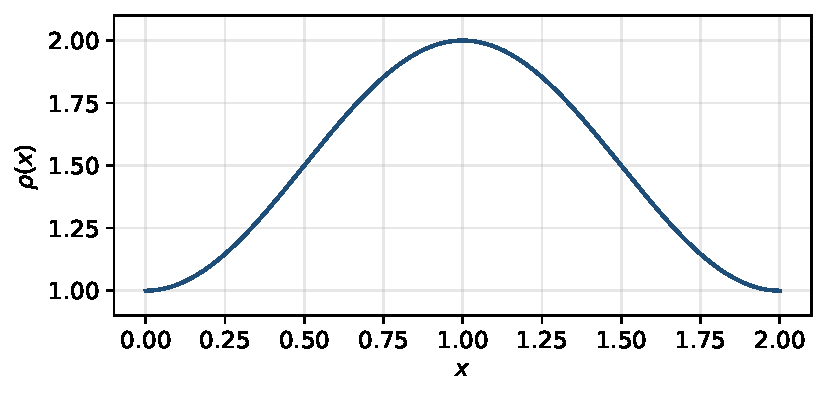
\includegraphics[width=0.62\textwidth]{figures/rho.pdf}
\caption{Коэффициент $\rho(x)=1+\sin^2(\pi x/2)$; максимум достигается
во внутренней точке $x=1$}
\label{fig:rho}
\end{figure}

\begin{figure}[htbp]
\centering
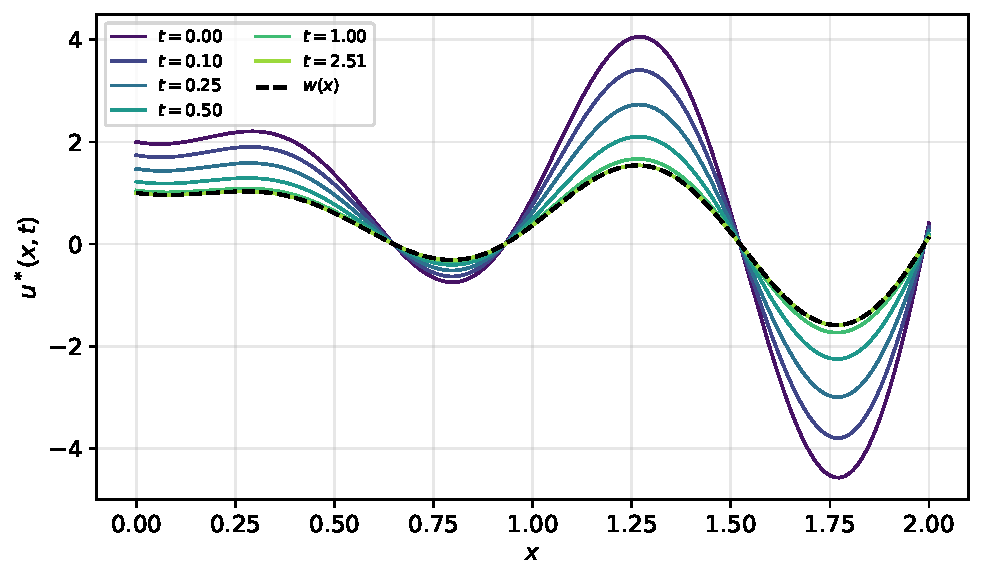
\includegraphics[width=0.8\textwidth]{figures/exact.pdf}
\caption{Точное решение $u^*(x,t)$ в разные моменты времени и
установившееся решение $w(x)$}
\label{fig:exact}
\end{figure}

\subsection{Явная схема: число разбиений (задание 1а)}
\label{sec:M0}

Число разбиений $M_0$ ищется при выполнении условия
устойчивости~\eqref{eq:stabcond}: на каждой сетке берётся максимально
допустимый шаг $\tau=h^2/(2\rho_{\max})$. Тогда $\tau$ сам
пропорционален $h^2$, и по~\eqref{eq:orders} погрешность остаётся
$O(h^2)$. Это подтверждается табл.~\ref{tab:conv} и рис.~\ref{fig:conv}:
точки ложатся на прямую с угловым коэффициентом 2.

\begin{table}[htbp]
\caption{Погрешность явной схемы при $\tau=h^2/(2\rho_{\max})$}
\label{tab:conv}
\centering
\begin{tabular}{r c c r c}
\toprule
$M$ & $h$ & $\tau$ & $N$ & $\varepsilon$\\
\midrule
20 & $0.10000$ & $2.500\cdot10^{-3}$ & 1006 & $2.293\cdot10^{-1}$ \\
30 & $0.06667$ & $1.111\cdot10^{-3}$ & 2263 & $1.136\cdot10^{-1}$ \\
40 & $0.05000$ & $6.250\cdot10^{-4}$ & 4023 & $6.618\cdot10^{-2}$ \\
60 & $0.03333$ & $2.778\cdot10^{-4}$ & 9050 & $3.032\cdot10^{-2}$ \\
80 & $0.02500$ & $1.563\cdot10^{-4}$ & 16089 & $1.736\cdot10^{-2}$ \\
120 & $0.01667$ & $6.944\cdot10^{-5}$ & 36200 & $7.840\cdot10^{-3}$ \\
160 & $0.01250$ & $3.906\cdot10^{-5}$ & 64356 & $4.444\cdot10^{-3}$ \\
240 & $0.00833$ & $1.736\cdot10^{-5}$ & 144799 & $1.989\cdot10^{-3}$ \\
\bottomrule
\end{tabular}
\end{table}

\begin{figure}[htbp]
\centering
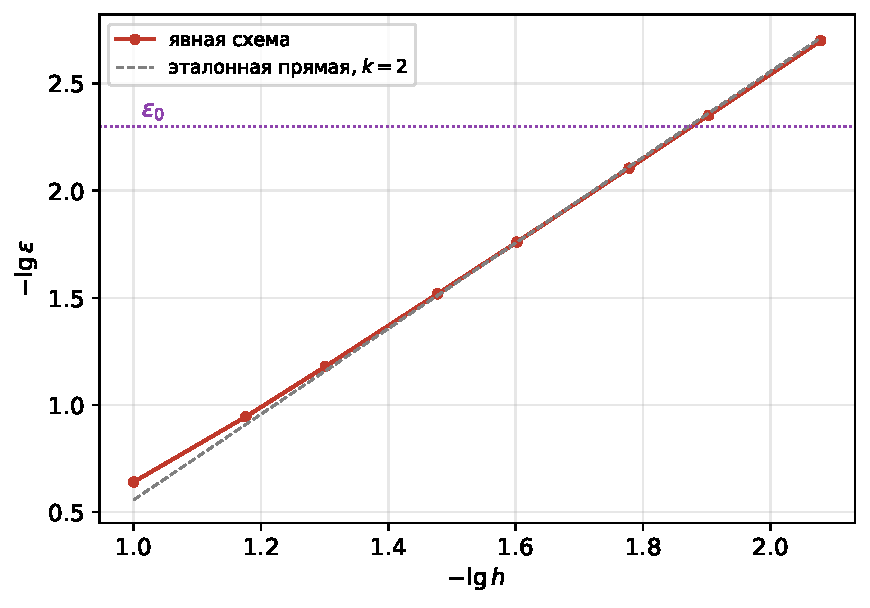
\includegraphics[width=0.68\textwidth]{figures/convergence.pdf}
\caption{Погрешность явной схемы в зависимости от шага сетки;
штриховая --- эталонная прямая с наклоном $k=2$, пунктир --- заданная
точность $\varepsilon_0$}
\label{fig:conv}
\end{figure}

Так как $\varepsilon(M)$ монотонно убывает, $M_0$ находится двоичным
поиском: сначала сетка удваивается до выполнения
$\varepsilon<\varepsilon_0$, затем вилка сужается. Это заметно дешевле
перебора: стоимость одного прогона растёт как $M^3$, потому что число
шагов по времени само пропорционально $M^2$. Получено
\begin{equation}\label{eq:M0}
M_0=151,\qquad h_0=0{,}013245,\qquad
\tau_0=\frac{h_0^2}{2\rho_{\max}}=4{,}3858\cdot10^{-5},
\end{equation}
причём требуемое условие выполнено:
\[
\varepsilon(M_0)=4{,}983\cdot10^{-3}<\varepsilon_0=5\cdot10^{-3}
<\varepsilon(M_0-1)=5{,}047\cdot10^{-3}.
\]
Число шагов по времени при этом $N=57\,319$.

\subsection{Явная схема: счёт до момента установления (задание 1б)}

Расчёт с найденными $h_0$ и $\tau_0$ доведён до $t=T$. Текущее решение
выводится на экран в реальном времени, и одновременно на экране «висит»
установившееся решение $w(x)$ (программа \texttt{anim.py}). Несколько
кадров этого расчёта собраны на рис.~\ref{fig:explicit}: решение
монотонно подходит к $w(x)$, в согласии с точным
решением~\eqref{eq:ustar}.

\begin{figure}[htbp]
\centering
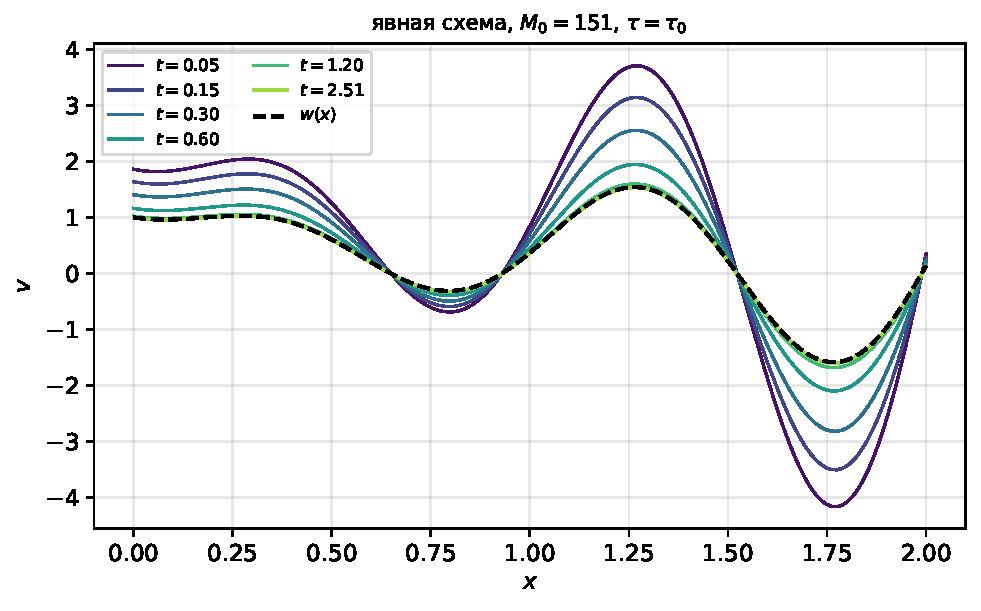
\includegraphics[width=0.8\textwidth]{figures/explicit.pdf}
\caption{Явная схема при $M_0=151$, $\tau=\tau_0$: численное решение в
разные моменты и установившееся решение $w(x)$ (штриховая)}
\label{fig:explicit}
\end{figure}

\subsection{Явная схема: развитие неустойчивости (задание 1в)}
\label{sec:instab}

Положим $\tau=\tau_0+\Delta\tau$ с $\Delta\tau=0{,}02\,\tau_0$. Счёт
разрушается: решение перестаёт иметь отношение к задаче уже при
$t\approx0{,}07$ из требуемых $2{,}51$.

Картина полностью объясняется теорией (рис.~\ref{fig:instab}). Справа
показан профиль погрешности перед разрушением: это пила, меняющая знак
от узла к узлу, то есть самая короткая гармоника $\varphi=\pi$, для
которой множитель перехода $\lambda=1-4r$ по модулю первым превышает
единицу. Пила сосредоточена около $x=1$ --- там, где $\rho$ максимален
и, значит, максимален $r_i$.

Слева --- рост погрешности во времени в логарифмическом масштабе. Чтобы
сравнить наблюдаемый рост с теоретическим, оценки $|1-4r|$ с
замороженным коэффициентом недостаточно: она не учитывает ни
переменности $\rho$, ни краевых уравнений. Поэтому построена матрица
перехода $G$ полной задачи:
\[
G_{i,i-1}=r_i,\qquad G_{i,i}=1-2r_i,\qquad G_{i,i+1}=r_i
\qquad (i=1,\dots,M-1),
\]
а строки $0$ и $M$ получаются подстановкой уже пересчитанных внутренних
значений в краевые уравнения~\eqref{eq:bc_h}. Счёт устойчив тогда и
только тогда, когда $\lambda_{\max}=\max|\mathrm{eig}\,G|\le1$.
Наблюдаемый множитель роста за шаг и спектральный радиус совпадают с
точностью до семи знаков:
\[
\text{наблюдение } 1{,}0250495,\qquad \lambda_{\max}=1{,}0250497 .
\]

\begin{figure}[htbp]
\centering
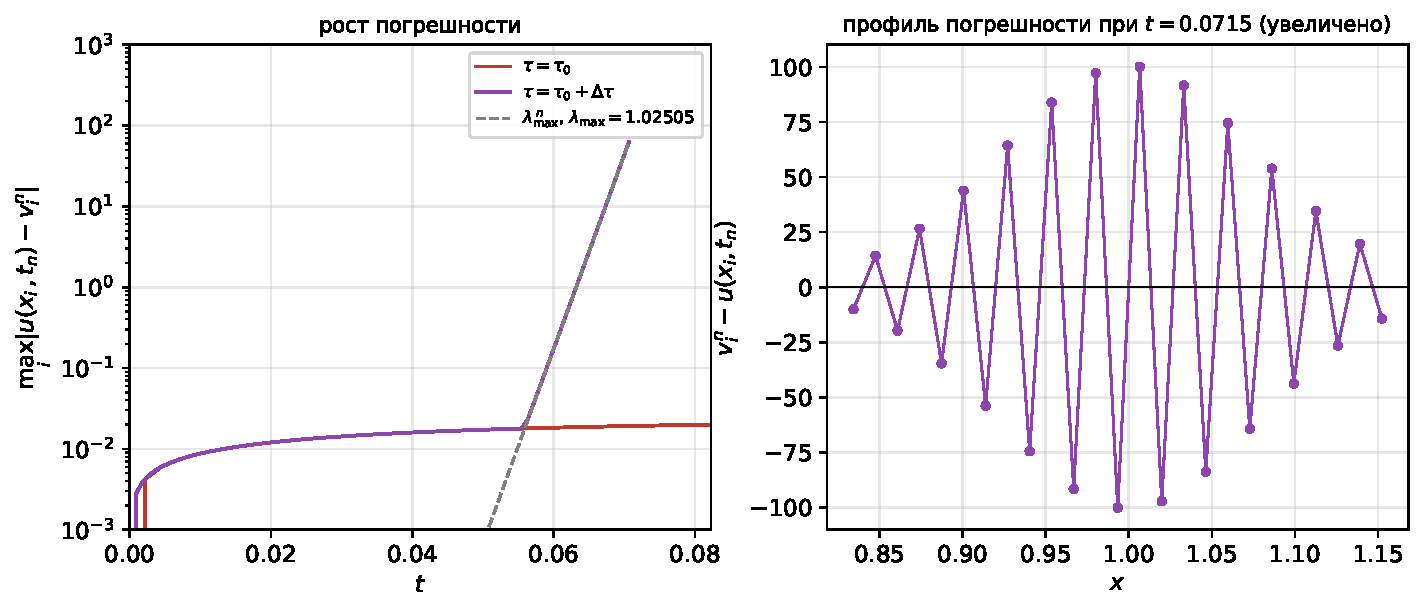
\includegraphics[width=\textwidth]{figures/instability.pdf}
\caption{Развитие неустойчивости явной схемы при
$\tau=\tau_0+\Delta\tau$: слева рост погрешности и теоретическая прямая
$\lambda_{\max}^{\,n}$, справа пилообразный профиль погрешности перед
разрушением}
\label{fig:instab}
\end{figure}

Табл.~\ref{tab:stab} сопоставляет спектральный радиус и исход счёта.
Порог лежит чуть выше $\tau_0$: по спектру граница равна
$1{,}0074\,\tau_0$. Это не противоречит условию~\eqref{eq:stabcond} ---
оно \emph{достаточное}. Запас в $0{,}7\%$ возникает потому, что
неустойчивая гармоника должна уместиться в окрестности точки $x=1$, где
$\rho$ близок к $\rho_{\max}$, а локализация снижает скорость роста.
Для практики существенно, что уже при $\tau=1{,}01\,\tau_0$ счёт
разрушается.

\begin{table}[htbp]
\caption{Спектральный радиус матрицы перехода явной схемы и исход счёта
($M_0=151$)}
\label{tab:stab}
\centering
\begin{tabular}{c c c}
\toprule
$\tau/\tau_0$ & $\lambda_{\max}$ & результат счёта\\
\midrule
0.95 & 0.999942 & устойчиво \\
0.99 & 0.999939 & устойчиво \\
1.00 & 0.999939 & устойчиво \\
1.01 & 1.005196 & разрушение \\
1.02 & 1.025050 & разрушение \\
1.05 & 1.084610 & разрушение \\
\bottomrule
\end{tabular}
\end{table}

\subsection{Неявная схема (задание 2)}

Та же задача решена неявной схемой. При $\tau=\tau_0$ результат
практически совпадает с явной схемой ($\varepsilon=4{,}989\cdot10^{-3}$
против $4{,}983\cdot10^{-3}$): при таком мелком шаге по времени
погрешность целиком определяется пространственной аппроксимацией.

Главное отличие --- поведение при $\tau=\tau_0+\Delta\tau$, на котором
явная схема разрушилась. Неявная схема считает без каких-либо признаков
неустойчивости и даёт ту же точность $\varepsilon=4{,}989\cdot10^{-3}$
(рис.~\ref{fig:implicit}). Это прямое подтверждение безусловной
устойчивости, доказанной в п.~\ref{sec:stab}: при $\theta\ge1/2$
неравенство $|\lambda|\le1$ выполняется при любом $s$, то есть при
любом $\tau$.

\begin{figure}[htbp]
\centering
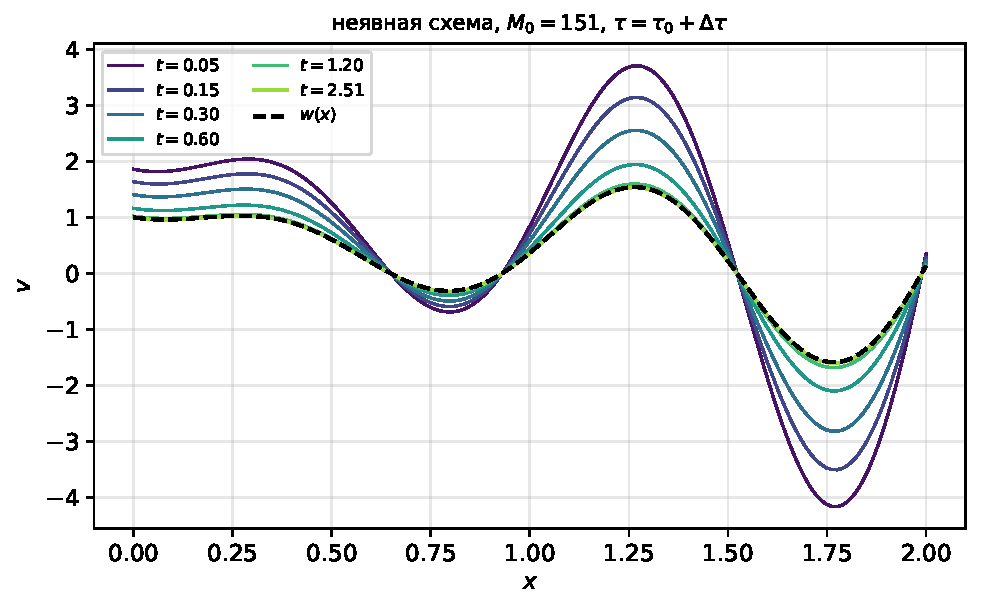
\includegraphics[width=0.8\textwidth]{figures/implicit.pdf}
\caption{Неявная схема при $M_0=151$, $\tau=\tau_0+\Delta\tau$ --- при
том же шаге, на котором явная схема разрушается, счёт идёт устойчиво}
\label{fig:implicit}
\end{figure}

\subsection{Увеличение шага по времени (задания 4 и 5.3)}
\label{sec:taustar}

Значение $\tau_0$ продиктовано устойчивостью явной схемы, а не
точностью. Неявная и симметричная схемы устойчивы безусловно, поэтому
естественно спросить, насколько можно увеличить $\tau$ при том же
$h_0$, не выходя за $\varepsilon_0$. Величина $\tau^*$ ищется так же,
как $M_0$: шаг удваивается до нарушения неравенства, затем граница
уточняется двоичным поиском.

Сразу отметим, что запас по точности невелик: по построению
$\varepsilon(M_0)=4{,}983\cdot10^{-3}$ лежит лишь на $0{,}35\%$ ниже
$\varepsilon_0$, и весь этот запас можно «потратить» на увеличение
$\tau$.

\paragraph{Неявная схема.} Результаты --- в табл.~\ref{tab:epstau_imp} и
на левой панели рис.~\ref{fig:epstau}. Погрешность растёт линейно по
$\tau$, как и предсказывает~\eqref{eq:orders}, и обе оценки погрешности
(по $\Omega_{h\tau}$ и по контрольным моментам) совпадают. Получено
\[
\tau^*=2{,}09\cdot10^{-4}=4{,}8\,\tau_0 ,
\]
то есть шаг можно увеличить почти в пять раз; число шагов падает с
$57\,319$ до $12\,008$.

\begin{table}[htbp]
\caption{Неявная схема: погрешность в зависимости от шага по времени
($M_0=151$)}
\label{tab:epstau_imp}
\centering
\begin{tabular}{c c r c c}
\toprule
$\tau$ & $\tau/\tau_0$ & $N$ & $\varepsilon$ &
$\varepsilon_{\text{к}}$\\
\midrule
$4.386\cdot10^{-5}$ & 1.00 & 57319 & $4.9888\cdot10^{-3}$ & $4.9886\cdot10^{-3}$ \\
$5.827\cdot10^{-5}$ & 1.33 & 43140 & $4.9898\cdot10^{-3}$ & $4.9896\cdot10^{-3}$ \\
$7.743\cdot10^{-5}$ & 1.77 & 32468 & $4.9911\cdot10^{-3}$ & $4.9909\cdot10^{-3}$ \\
$1.029\cdot10^{-4}$ & 2.35 & 24436 & $4.9928\cdot10^{-3}$ & $4.9926\cdot10^{-3}$ \\
$1.367\cdot10^{-4}$ & 3.12 & 18391 & $4.9951\cdot10^{-3}$ & $4.9949\cdot10^{-3}$ \\
$1.816\cdot10^{-4}$ & 4.14 & 13842 & $4.9981\cdot10^{-3}$ & $4.9979\cdot10^{-3}$ \\
$2.094\cdot10^{-4}$ & 4.77 & 12008 & $5.0000\cdot10^{-3}$ & $4.9997\cdot10^{-3}$ \\
\bottomrule
\end{tabular}
\end{table}

\paragraph{Симметричная схема.} Здесь формальный ответ требует
оговорки. Данные --- в табл.~\ref{tab:epstau_sym} и на правой панели
рис.~\ref{fig:epstau}.

По определению~\eqref{eq:eps_max} неравенство
$\varepsilon\le\varepsilon_0$ держится вплоть до
$\tau=2{,}82\cdot10^{-1}=6436\,\tau_0$, причём $\varepsilon$ при росте
$\tau$ сначала даже \emph{убывает}. Это не улучшение решения: при
$\tau=0{,}28$ на весь расчёт приходится всего 9 слоёв по времени.
Максимум погрешности достигается на переходном участке, а редкая сетка
$\Omega_\tau$ туда просто не попадает --- ровно та ситуация, ради
которой введена контрольная оценка. Контрольная оценка ведёт себя
монотонно и при $\tau=0{,}28$ даёт
$\varepsilon_{\text{к}}=3{,}8\cdot10^{-2}$, то есть в восемь раз хуже
требуемого.

Поэтому за рабочее значение принимается граница по контрольной оценке:
\[
\tau^{**}=4{,}97\cdot10^{-2}=1134\,\tau_0 ,
\]
при ней расчёт занимает 51 шаг вместо $57\,319$. Выигрыш по сравнению с
неявной схемой --- ещё примерно в 230 раз, и он объясняется
порядком~\eqref{eq:orders}: у симметричной схемы временная погрешность
$O(\tau^2)$, а не $O(\tau)$.

\begin{table}[htbp]
\caption{Симметричная схема: погрешность в зависимости от шага по
времени ($M_0=151$)}
\label{tab:epstau_sym}
\centering
\begin{tabular}{c r r c c}
\toprule
$\tau$ & $\tau/\tau_0$ & $N$ & $\varepsilon$ &
$\varepsilon_{\text{к}}$\\
\midrule
$4.386\cdot10^{-5}$ & 1 & 57319 & $4.9857\cdot10^{-3}$ & $4.9855\cdot10^{-3}$ \\
$2.160\cdot10^{-4}$ & 5 & 11637 & $4.9852\cdot10^{-3}$ & $4.9850\cdot10^{-3}$ \\
$1.064\cdot10^{-3}$ & 24 & 2363 & $4.9824\cdot10^{-3}$ & $4.9823\cdot10^{-3}$ \\
$5.242\cdot10^{-3}$ & 120 & 480 & $4.9682\cdot10^{-3}$ & $4.9677\cdot10^{-3}$ \\
$1.163\cdot10^{-2}$ & 265 & 217 & $4.9453\cdot10^{-3}$ & $4.9392\cdot10^{-3}$ \\
$2.582\cdot10^{-2}$ & 589 & 98 & $4.8830\cdot10^{-3}$ & $4.8643\cdot10^{-3}$ \\
$4.974\cdot10^{-2}$ & 1134 & 51 & $4.7518\cdot10^{-3}$ & $4.9999\cdot10^{-3}$ \\
$1.272\cdot10^{-1}$ & 2900 & 20 & $4.1505\cdot10^{-3}$ & $1.0248\cdot10^{-2}$ \\
$2.823\cdot10^{-1}$ & 6436 & 9 & $4.9968\cdot10^{-3}$ & $3.8215\cdot10^{-2}$ \\
\bottomrule
\end{tabular}
\end{table}

\begin{figure}[htbp]
\centering
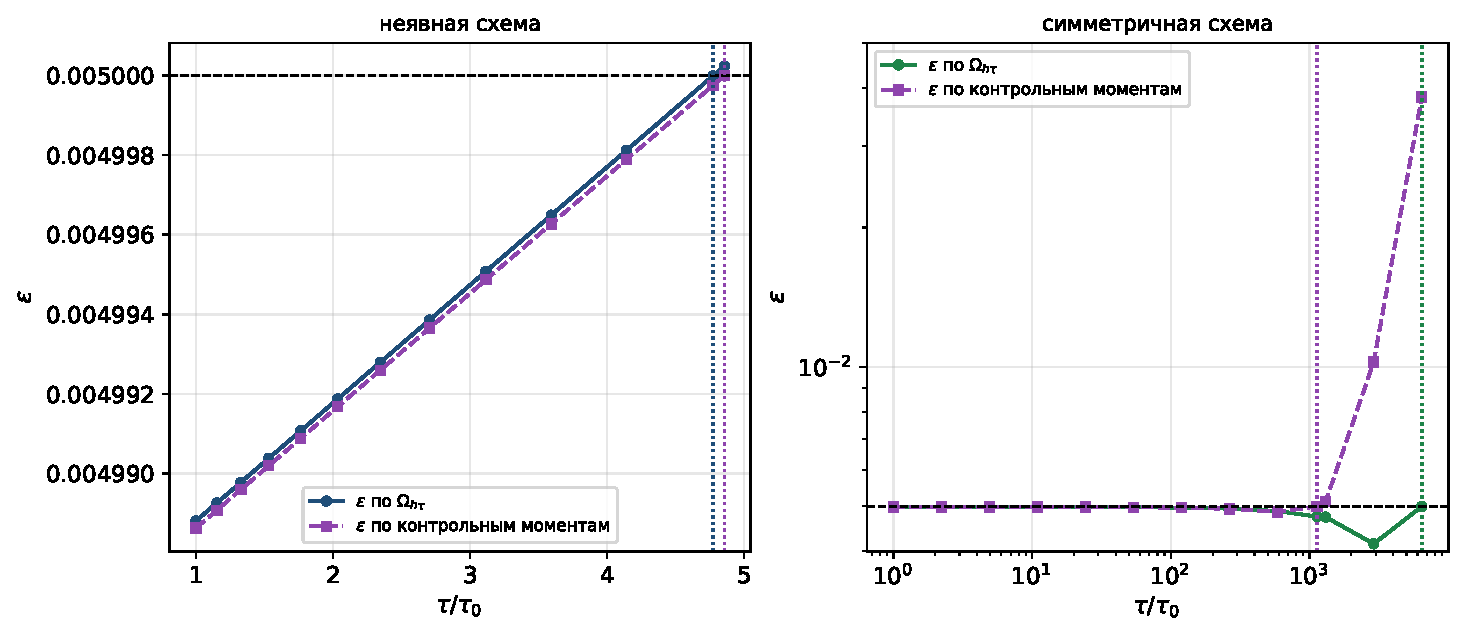
\includegraphics[width=\textwidth]{figures/eps_tau.pdf}
\caption{Зависимость погрешности от шага по времени при $h=h_0$.
Горизонтальная штриховая --- $\varepsilon_0$, вертикальные пунктиры ---
границы по двум оценкам погрешности}
\label{fig:epstau}
\end{figure}

Расчёты с найденными шагами доведены до $t=T$; рис.~\ref{fig:impstar}
и~\ref{fig:symstar} показывают, что решение по-прежнему выходит на
установившийся режим.

\begin{figure}[htbp]
\centering
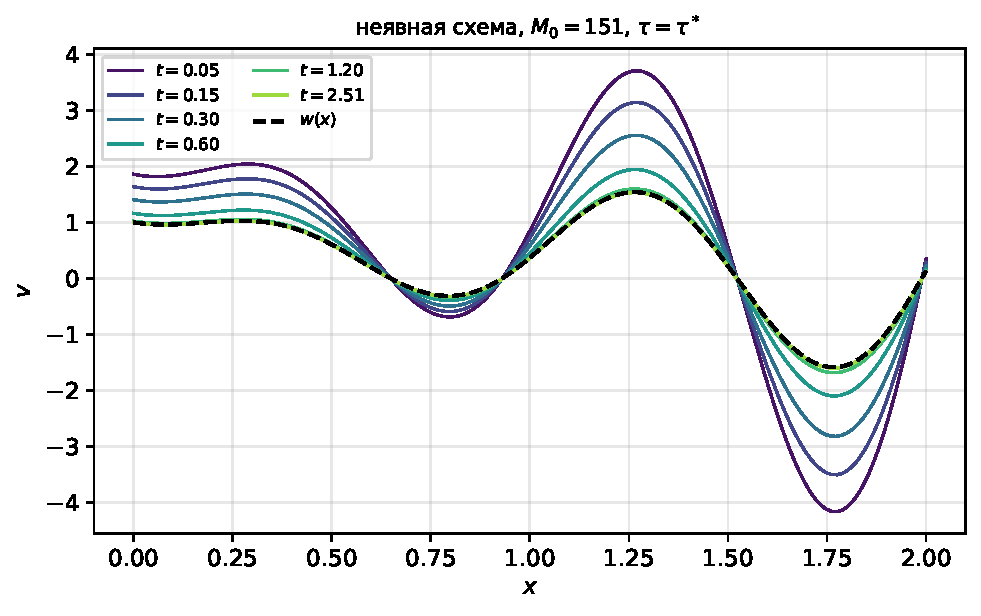
\includegraphics[width=0.8\textwidth]{figures/implicit_star.pdf}
\caption{Неявная схема при $M_0=151$, $\tau=\tau^*=4{,}8\,\tau_0$}
\label{fig:impstar}
\end{figure}

\begin{figure}[htbp]
\centering
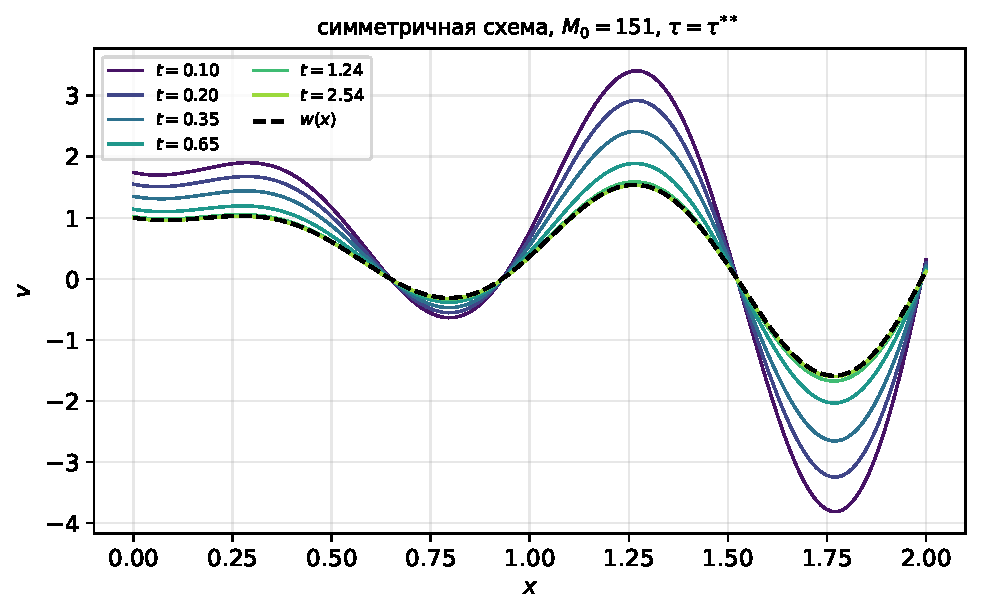
\includegraphics[width=0.8\textwidth]{figures/symmetric_star.pdf}
\caption{Симметричная схема при $M_0=151$,
$\tau=\tau^{**}=1134\,\tau_0$ (всего 51 шаг по времени)}
\label{fig:symstar}
\end{figure}

\subsection{Трудоёмкость схем (задание 5.4)}
\label{sec:cost}

Сравним схемы при $h=h_0$, каждую --- с её максимально допустимым шагом
по времени. Оценим сначала число арифметических операций на один шаг,
считая по $M$ узлам:

\begin{itemize}
\item \emph{явная}: разностное отношение --- 3 операции, умножение на
      $r_i$ --- 1, вычисление $f$ --- 2, умножение на $\tau$ --- 1, два
      сложения --- 2; итого $\approx9M$;
\item \emph{неявная}: правая часть $\approx4M$ плюс прогонка с готовыми
      прогоночными коэффициентами (прямой ход 2 операции на узел,
      обратный 3) --- $5M$; итого $\approx9M$;
\item \emph{симметричная}: то же плюс разностный оператор на старом слое
      --- ещё $\approx7M$; итого $\approx16M$.
\end{itemize}

Стоимость одного шага у явной и неявной схем практически одинакова, у
симметричной примерно вдвое выше. Поэтому полная трудоёмкость
определяется числом шагов (табл.~\ref{tab:cost}).

\begin{table}[htbp]
\caption{Трудоёмкость схем при $h=h_0$ ($M_0=151$)}
\label{tab:cost}
\centering
\begin{tabular}{l c r c c c}
\toprule
схема & $\tau/\tau_0$ & $N$ & операций & время, с & $\varepsilon$\\
\midrule
явная & 1.0 & 57319 & $7{,}8\cdot10^{7}$ & 1.40 & $4.983\cdot10^{-3}$\\
неявная & 4.9 & 11805 & $1{,}6\cdot10^{7}$ & 2.24 & $5.000\cdot10^{-3}$\\
симметричная & 1134.0 & 51 & $1{,}2\cdot10^{5}$ & 0.01 & $4.752\cdot10^{-3}$\\
\bottomrule
\end{tabular}
\end{table}

По числу операций неявная схема дешевле явной примерно в 5 раз, а
симметричная --- в 630 раз. Измеренное время у неявной схемы при этом
\emph{больше}, чем у явной, и это не противоречие, а свойство
реализации: явный шаг --- одна векторная операция \texttt{numpy} над
массивом из 152 чисел, тогда как прогонка содержит два последовательных
цикла на языке Python, и накладные расходы интерпретатора на узел
существенно выше. Оценка по числу операций от этого свободна, поэтому
именно она характеризует трудоёмкость самих схем; измеренное время
приведено для полноты. Для симметричной схемы расхождения нет: выигрыш
в три порядка перекрывает любую разницу в стоимости шага.

\section{Выводы}

\begin{enumerate}
\item Для краевой задачи третьего рода~\eqref{eq:pde}--\eqref{eq:bc}
построены и реализованы три разностные схемы --- явная, неявная и
симметричная. Все три записываются одной схемой с весом $\theta$ и
отличаются только его значением; краевые условия во всех случаях
аппроксимированы по $x$ со вторым порядком трёхточечной односторонней
разностью, поэтому сравнение схем не искажается разной обработкой
границы. Неявная и симметричная схемы приводят к системе линейных
алгебраических уравнений (СЛАУ) с трёхдиагональной матрицей, которая
решается методом прогонки; прогоночные коэффициенты вычисляются один
раз, так как матрица от номера слоя не зависит.

\item Теоретические порядки аппроксимации подтвердились. При счёте
явной схемой с максимально допустимым шагом $\tau=h^2/(2\rho_{\max})$
погрешность убывает как $O(h^2)$ (рис.~\ref{fig:conv}), что отвечает
оценке~\eqref{eq:orders}, в которой $\tau$ сам пропорционален $h^2$.
Заданная точность $\varepsilon_0=5\cdot10^{-3}$ достигается при
$M_0=151$, причём $\varepsilon(M_0)<\varepsilon_0<\varepsilon(M_0-1)$.

\item Граница устойчивости явной схемы подтверждена количественно.
Условие $\tau\le h^2/(2\rho_{\max})$, полученное и принципом максимума,
и спектральным признаком, является достаточным; точная граница,
найденная по спектральному радиусу матрицы перехода, равна
$1{,}0074\,\tau_0$. При $\tau=1{,}02\,\tau_0$ счёт разрушается к
$t\approx0{,}07$, погрешность растёт как пила с периодом в два шага
сетки, сосредоточенная около точки максимума $\rho$, а наблюдаемый
множитель роста совпадает со спектральным радиусом до семи знаков.

\item Безусловная устойчивость неявной и симметричной схем
($\theta\ge1/2$) подтверждена прямым счётом: при том же
$\tau=\tau_0+\Delta\tau$, на котором разрушается явная схема, они дают
ту же точность, что и при $\tau=\tau_0$.

\item Шаг по времени, продиктованный устойчивостью, оказался намного
меньше, чем требуется для заданной точности. При $h=h_0$ его можно
увеличить в $4{,}8$ раза для неявной схемы и примерно в $1100$ раз для
симметричной, не выходя за $\varepsilon_0$. Разница между схемами
отвечает порядку по времени: $O(\tau)$ против $O(\tau^2)$.

\item Формальное определение погрешности~\eqref{eq:eps_max} при больших
$\tau$ перестаёт быть надёжным, поскольку сеточная область
$\Omega_\tau$ сама зависит от $\tau$ и при малом числе слоёв не
захватывает момент наибольшей погрешности. Для симметричной схемы это
приводит к немонотонной зависимости $\varepsilon(\tau)$ и завышенной
границе $6436\,\tau_0$ вместо $1134\,\tau_0$ по контрольной оценке.

\item По числу арифметических операций неявная схема дешевле явной
примерно в 5 раз, симметричная --- в 630 раз; стоимость одного шага у
явной и неявной схем одинакова, у симметричной выше примерно вдвое, так
что весь выигрыш даёт сокращение числа шагов.
\end{enumerate}

\end{document}
